\protect \section *{\protect \nameref  *{QuasiStationarMedia}}
\begin{Solution}{7.{2}}
	Передусім відзначимо, що тут ми розглядаємо ідеальну картину з неперервним рівномірним розподілом густини заряду, як це зазвичай прийнято в макроскопічній електродинаміці. Виберемо систему декартових координат з абсцисою ортогонально до початкового шару.

	Нехай $X(x,t)$~--- траєкторія частинки, яка при $t = 0$   мала координату $x$ , тобто $X(0,t) = x$. Напруженість поля зростає монотонно по $x$, відповідно, швидкість і прискорення кожної частинки~--- також. Тому <<задні>> частинки не наздоганяють <<передні>>, тобто  $X(x_1,t) > X(x_2,t)$  при ${x_1} > {x_2}$.

		Оскільки поле плаского шару ~--- однорідне у просторі, це означає, що на кожну частинку весь час діє одне і теж саме електричне поле:
		\[
			\frac{{{\partial ^2}X(x,t)}}{{\partial {t^2}}} = \frac{e}{m_e}E(x) = \omega _p^2x,
		\]
		\[
			\omega _p^2 = \frac{{4\pi {e^2}{n_0}}}{m_e},
		\]
	$m_e$~--- маса електрона. Поле однорідного шару визначено за теоремою Гаусса.

		З рівнянь рівноприскореного руху:
		\[
			X(x,t) = x\left[ {1 + \omega _p^2\frac{{{t^2}}}{2}} \right]
		\]
		видно, що розподіл частинок весь час пропорційний початковому положенню.

		Положення крайніх частинок $X(a,t) = a\left[ {1 + \omega _p^2\frac{{{t^2}}}{2}} \right]$.
	Густина у будь-якій точці шару, що розширюється, є
	\[
		\rho (x,t) = e{n_0}{\left[ {1 + \omega _p^2\frac{{{t^2}}}{2}} \right]^{ - 1}}\theta \left[ {X(a,t) - x} \right].
	\]
\end{Solution}
\begin{Solution}{7.{3}}
	Всередині плити відбувається розтікання заряду (максвелівська релаксація), яке має місце за умови виконання закону Ома. А саме, з рівняння неперервності, закону Ома та рівняння Максвелла $\vect{\nabla}\cdot\Efield = -4\pi\rho$   випливає:
	\[
		\rho (x,t) = \rho_1\exp \left(  - \frac{4\pi \lambda _1}{\epsilon _1}t \right).
	\]

	Для плаского розподілу заряду поле спрямовано по осі $x$. З рівняння Максвелла маємо:
	\[
		E_x(x,t) = 4\pi \left( {x - \frac{a}{2}} \right)\frac{{{\rho_1}}}{{{\epsilon _1}}}\exp \left( { - \frac{{4\pi {\lambda _1}}}{{{\epsilon_1}}}t} \right),
	\]
	звідки, за законом Ома:
	\[
		\vect{j}(x,t) = 4\pi \vect{e}_x\left( x - \frac{a}{2} \right)\frac{\lambda _1\rho _1}{\epsilon _1}\exp \left( - \frac{4\pi\lambda_1}{\epsilon_1}t \right).
	\]

	Заряд, що був всередині, з часом порівну розподіляється між двома поверхнями плити і на кожній з них

	\[
		\sigma (t) = \frac{a\rho_1}{2}\left[ {1 - \exp \left( { - \frac{{4\pi {\lambda _1}}}{{{\varepsilon _1}}}t} \right)} \right].
	\]
	%Звідси видно, що знак $\sigma(t)$  за малих $t$ визначається співвідношенням  $\lambda_1/\epsilon_1$ і  $\lambda_2/\epsilon_2$. Наприклад, якщо середовище зовні плити ізолятор $\lambda _2/\epsilon_2 \ll  \lambda_1/\epsilon_1$, спочатку майже весь заряд зосереджується на поверхні, а потім повільно спадає.
\end{Solution}
\begin{Solution}{7.{4}}
	Задача аналогічна~\ref{prb:MaxwellRelax}. З урахуванням циліндричної симетрії задачі видно, що напруженість електричного поля має лише радіальну (перпендикулярну до осі циліндра) компоненту. З інтегральної форми рівнянь Максвелла в середовищі маємо:
	\[
		\Efield({\vect{r}},t) = 2\pi {\vect{r}}\frac{{{\rho _1}}}{{{\epsilon _1}}}\exp \left( { - \frac{{4\pi {\lambda _1}}}{{{\epsilon_1}}}t} \right),
	\]
	звідки
	\[
		\vect{j}(\vect{r},t) = 2\pi \vect{r}\frac{{{\lambda_1}{\rho_1}}}{{{\epsilon_1}}}\exp \left( { - \frac{{4\pi {\lambda _1}}}{{{\epsilon _1}}}t} \right).
	\]
	Для поверхневої густини заряду маємо:
	\[
		\sigma (t) = \frac{{R{\rho _1}}}{2}\left[ {1 - \exp \left( { - \frac{{4\pi {\lambda _1}}}{{{\varepsilon _1}}}t} \right)} \right].
	\]
\end{Solution}
\begin{Solution}{7.{5}}
	Всередині кулі маємо:
	\[
		\rho (t) = {\rho _1}\exp \left( { - \frac{{4\pi {\lambda_1}}}{{{\varepsilon _1}}}t} \right).
	\]
	Заряд зосереджується на поверхні кулі з густиною:
	\[
		\sigma (t) = \frac{{R{\rho _1}}}{3}\left[ {1 - \exp \left( { - \frac{{4\pi {\lambda _1}}}{{{\varepsilon _1}}}t} \right)} \right].
	\]
	З урахуванням сферичної симетрії задачі (напруженість електричного в окремій точці спрямована по радіусу) та з інтегральної форми рівнянь Максвелла в середовищі отримуємо напруженість поля. Густина струму:
	\[
		\vect{j}(\vect{r},t) = 4\pi \vect{r}\frac{{{\lambda_1}{\rho _1}}}{{3{\epsilon _1}}}\exp \left( { - \frac{{4\pi {\lambda_1}}}{{{\epsilon _1}}}t} \right).
	\]
\end{Solution}
\begin{Solution}{7.{7}}
    Використавши  рівняння для електричного поля~\label{eq:skin-effect} в циліндричних координатах та закон Ома отримаємо рівняння для густини струму:
\[
		\frac{1}{r}\frac{\partial }{{\partial r}}\left( {r\frac{{\partial {j_z}}}{{\partial r}}} \right) + {k^2}{j_z} = 0, \quad k^2 = \frac{4i\pi\lambda\mu\omega}{c^2} = \frac{2i}{\delta^2}.
\]

Розв'язком цього рівняння є функція вигляду $j_z = AJ_0(kr) + BN_0(kr)$. Оскільки $\lim\limits_{r\to0}N_0(kr) = -\infty$, то стала $B = 0$. Сталу $A$ можна знайти знаючи амплітуду струму
\[
   I_0 = \int\limits_0^a j_z(r)\ 2\pi rdr = 2\pi A \int\limits_0^a r J_0(kr) dr = 2\pi A \frac{a}{k} J_1(ka),
\]
отже, густина струму
\[
	j_z = \frac{k}{2\pi a} \frac{J_0(kr)}{J_1(ka)} I_0e^{-i\omega t}.
\]
За великих частот $ka \gg 1$ та в області біля краю провідника $ r \lessapprox a$ (див. формулу~\eqref{eq:Jxgg1}) маємо:
\[
    j_z = \frac{1-i}{2\pi\delta} I_0 \sqrt{\frac1{ar}} e^{\left( \frac{i - 1}{\delta} (a-r) - i\omega t\right) }.
\]

Дійсна амплітуда густини струму має вигляд:
\[
    j_0(r) = \frac{I_0\sqrt{2}}{2\pi\delta}  \sqrt{\frac1{ar}}e^{\frac{r-a}{\delta}},
\]
графічне зображення зображення цієї залежності подано на рисунку

\begin{center}
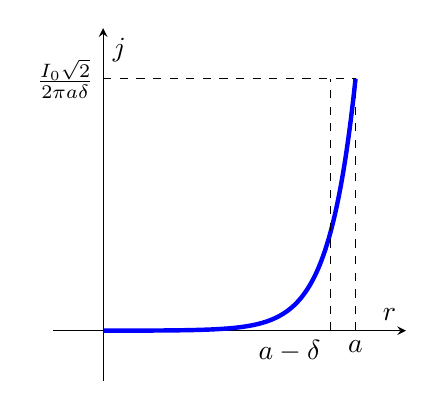
\begin{tikzpicture}
\begin{axis}%
[
            clip=false,
			axis lines = middle,
			axis line style={-stealth},
			% === Підпис координатних осей ===
            xtick = \empty,
            ytick = \empty,
			xlabel={$r$},
			ylabel={$j$},
		    % === Налаштування розміру графіка ===
   			width=0.5\linewidth,
   			height=0.5\linewidth,
   			% === Розширення границь осей ===
   			enlargelimits={abs=0.2},
]

\addplot[blue, domain=0:1, samples=500, ultra thick] {sqrt(1/x)*e^(-(1-x)/(1e-1))};
\draw[dashed] (axis cs:1,0) node[below] {$a$} -- (axis cs:1,1);
\draw[dashed] (axis cs:0.9,0) node[below left] {$a-\delta$} -- (axis cs:0.9,1);
\draw[dashed] (axis cs:0,1) node[left] {$\frac{I_0\sqrt{2}}{2\pi a\delta} $} -- (axis cs:1,1);
\end{axis}
\end{tikzpicture}
\end{center}
\end{Solution}
\begin{Solution}{7.{8}}
Густина струму в циліндричному провіднику (див. розв'язок до задачі~\ref{prb:TrueSkin})
\[
	j_z = \frac{k}{2\pi a} \frac{J_0(kr)}{J_1(ka)} I_0e^{-i\omega t}.
\]

Опір будемо шукати як $R = \frac{\left\langle Q \right\rangle }{\frac12I_0^2}$.


Із закону Джоуля-Ленца розрахуємо теплоту, яка виділяється в провіднику як%
%\footnote{Використано співвідношення \href{https://www.wolframalpha.com/input/?i=integrate+from+0+to+a+besselJ0\%28k*x\%29*besselJ0\%28Conjugate\%28k\%29*x\%29+x+dx}{$\int\limits_0^a  J_0(kr)J_0(k^*r) r dr = \frac{kJ_1(ka)J_0(k^*a) - k^*J_1(k^*a)J_0(ka)}{k^2-k^{*2}} $} (в додатках нема)}

\begin{multline*}
    \left\langle Q \right\rangle = \frac1{2\lambda}\int\limits_0^a \left| j_z^2\right| 2\pi r dr = \frac{2\pi}{2(2\pi a)^2} \frac{I_0^2}{\lambda} \frac{|k|^2}{J_1(ka)J_1(k^*a)}  \int\limits_0^a  J_0(kr)J_0(k^*r) r dr = \\
    = \frac{2\pi a}{2(2\pi a)^2} \frac{I_0^2}{\lambda} \frac{|k|^2}{J_1(ka)J_1(k^*a)} \frac{kJ_1(ka)J_0(k^*a) - k^*J_1(k^*a)J_0(ka)}{k^2-k^{*2}} =\\
    = \frac{2\pi a }{2(2\pi a)^2} \frac{I_0^2}{\lambda} \frac{|k|^2\delta^2}{4i}\left( \frac{kJ_0(k^*a)}{J_1(k^*a)} - \frac{k^*J_0(ka)}{J_1(ka)}\right) = \\ = \frac{2\pi a}{2(2\pi a)^2} \frac{I_0^2}{\lambda} \frac12  \left( \frac{k^*J_0(k^*a)}{J_1(k^*a)} + \frac{kJ_0(ka)}{J_1(ka)}\right) =  \frac{1}{4\pi a} \frac{I_0^2}{\lambda}  \mathrm{Re}\left(  \frac{kJ_0(ka)}{J_1(ka)} \right).
\end{multline*}

Отже
\[
    R = \frac{1}{2\pi a\lambda}  \mathrm{Re}\left[  \frac{kJ_0(ka)}{J_1(ka)} \right].
\]

Розглянемо випадок малих частот $|ka| \ll 1$:
\[
    R \approx \frac{1}{2\pi a\lambda}  \mathrm{Re} \left[k\left( 1 - \frac{k^2a^2}{4}\right)\frac{2}{ka}  \right] = \frac{1}{\pi a^2 \lambda}.
\]
Тобто, при малих частотах опір такий же, як і для для постійного струму.

Розглянемо випадок великих частот $|ka| \gg 1$:
\[
    R \approx \frac{1}{2\pi a\lambda} \mathrm{Re}\left[  ke^{k(r-a)} \right] \approx \frac{1}{2\pi a\lambda} \mathrm{Re}\left[  k(1-k(r-a)) \right] =  \frac{1}{2\pi a\delta\lambda}.
\]
З останньої формули випливає, що ефективна площа перерізу провідника в області великих частот дорівнює $2\pi a\delta$, тобто має дуже маленьку величину, зосереджену поблизу поверхні провідника.
\end{Solution}
\begin{Solution}{7.{9}}
    $B_{\phi_{\mathrm{in}}} = \frac{2}{cr} \int\limits_0^r j_z 2\pi r dt = \frac{2I}{ca} \frac{J_1(kr)}{J_1(ka)}$.
\end{Solution}
\begin{Solution}{7.{10}}
    Внутрішню індуктивність можна обчислити знаючи магнітне поле в середині провідника (див. відповідь до задачі~\ref{prb:BfieldTrueSkin})  виходячи з виразу $\frac{1}{4c^2}L_\mathrm{in}I^2 = \int\limits_0^a \frac{\left\langle  B_{\phi_{\mathrm{in}}}^2\right\rangle }{8\pi} 2\pi rdr$, маємо
    $L_\mathrm{in}  = -\frac{\delta^2}{2a}\left[ \frac{k^*J_0(ka)}{J_1(ka)} + \frac{kJ_0(k^*a)}{J_1(k^*a)}\right] $. За низьких частот $|ka| \ll 1$ внутрішня індуктивність  $L_\mathrm{in} = \frac12$, за великих частот $|ka| \gg 1$ --- $L_\mathrm{in} = \frac\delta a$.
\end{Solution}
\begin{Solution}{7.{12}}
	Соленоїд створює однорідне магнітне поле, напрямлене по осі Z  всередині нього. Зовні соленоїда поле дорівнює нулю. За наявності циліндра в ньому виникають індукційні струми, що течуть по колам в площинах, ортогональних осі циліндра. Цю систему струмів можна розглядати як систему коаксіальних соленоїдів, поле яких не дає внесок зовні провідного  циліндра.

	Звідси магнітне поле $\Bfield = \Hfield = B_0\vect{e}_z$ при $r \in [a,b]$, де $B_0 = \frac{4\pi}{c}nI$, а зовні соленоїда (при $r > b$) $\Bfield = 0$.

	Усередині циліндра магнітне поле також напрямлене по осі $OZ$. Залежність усіх полів та струмів від часу така ж, як струм через обмотку.

	З рівнянь для квазістаціонарного поля (див. <<Теоретичні відомості, ф-ла ~\eqref{eq:skin-effect}>>) отримуємо
	\[
		\frac{1}{r}\frac{\partial }{{\partial r}}\left( {r\frac{{\partial {H_z}}}{{\partial r}}} \right) + {k^2}{H_z} = 0, \quad k^2 = \frac{4i\pi\lambda\mu\omega}{c^2} = \frac{2i}{\delta^2},
	\]
	що зводиться до рівняння для функції Бесселя $J_0$. Звідси, з урахуванням граничних умов для магнітного поля при $r = a$  та $r = b$, маємо
	\[H_z =
		\begin{cases}
			\frac{4\pi}{c}\frac{J_0(kr)}{J_0(ka)}nI_0e^{-i\omega t}, \quad r <a \\
			nI_0e^{-i\omega t}, \quad a \le r \le b                             \\
			0, r > b.
		\end{cases}
	\]

	Зауважимо, що $J_0(ka) \neq 0$, оскільки  $k$~--- комплексне, а нулі функції Бесселя лежать на дійсній осі.  З розкладу для  $J_0$  видно, що в формулу входить саме степені $k^2$, тому знак $k$ тут несуттєвий.

	При $r < a$, $\vect{j} = \frac{c}{4\pi}\rot\Hfield = \frac{c}{4\pi}\frac{d{H_z}}{dr}\left[ \vect{e}_r \times \vect{e}_z \right]$, звідки
	\[
		\vect{j} = knI_0\frac{J_1(kr)}{J_0(ka)}e^{-i\omega t}\vect{e}_{\phi},
	\]
	де використано що $J'_0(x) = -J_1(x)$. Використовуючи закон Ома $\Efield = \frac{\vect{j}}{\lambda}$, отримуємо електричне поле в середині провідника.
	Для областей $r >a$ та $r >b$ електричне поле можна знайти з рівняння Максвелла
	\[
		\frac{1}{r}\frac{\partial }{{\partial r}}\left( {r{E_\varphi }} \right) = \frac{{i\omega }}{c}{B_z} = \frac{{i\omega }}{c}{B_0}(t).
	\]

	Остаточно маємо
	\[
		E_{\phi} =
		\begin{cases}
			\frac{kcB_0}{4\pi\lambda}\frac{J_1(ka)}{J_0(ka)}e^{-i\omega t}, \quad r <a                                                                                        \\
			\frac{k}{\lambda}\frac{J_1(ka)}{J_0(ka)}\frac{a}{r}nI_0e^{-i\omega t} + \frac{4i\pi\omega }{2c^2r}\left( r^2 - a^2\right) nI_0e^{-i\omega t}, \quad a \le r \le b \\
			\frac{k}{\lambda}\frac{J_1(ka)}{J_0(ka)}\frac{a}{r}nI_0e^{-i\omega t} + \frac{4i\pi\omega }{2c^2r}\left( b^2 - a^2\right)nI_0e^{-i\omega t} , \quad r > b.
		\end{cases}
	\]
\end{Solution}
\begin{Solution}{7.{13}}
		Розподіл полів і струму аналогічний задачі~\ref{prb:Bat379}, але тут немає соленоїду. Розв’язок шукаємо в циліндричних координатах у вигляді  $\Bfield(r) = f(r)\vect{e}_ze^{- i\omega t}$,  $\vect{e}_z$~--- одиничний вектор  осі $OZ$. Зовні циліндру є лише зовнішнє поле, тому  гранична умова для напруженості така $f(a) = B_0$ .

		Аналогічно до задачі~\ref{prb:Bat379} рівняння для магнітного поля за умови регулярності при $r = 0$ дає

		\[
			\Hfield(r) = \vect{e}_z{B_0}\frac{{{J_0}(kr)}}{{{J_0}(ka)}} e^{ - i\omega t},
		\]
		де $ k = \frac{1 + i}{\delta}$, $\delta = \frac{c}{\sqrt {2\pi \mu \lambda \omega}}$.

		Густину струму знайдемо з рівняння Максвела як
		\[
			\vect{j}=  - \frac{c}{4\pi}\frac{dH_z}{dr}\vect{e}_\phi = \vect{e}_\phi B_0\frac{kc}{4\pi }\frac{J_1(kr)}{J_0(ka)}e^{ - i\omega t}.
		\]

		Для малих частот $|ka| \ll 1$ (або $\delta \gg a$) маємо
		\[
			\vect{j} = \vect{e}_\phi\frac{\lambda \mu \omega ir}{{2c}}e^{ - i\omega t}.
		\]

		За високих частот $|ka| \gg 1$ (або $\delta \ll a$) в області $r \gg \delta$
		\[
			\vect{j}=  \vect{e}_\phi\frac{{c{B_0}(i - 1)}}{{4\pi \delta }}\sqrt {\frac{a}{r}} \exp \left[ { - \frac{{a - r}}{\delta }(1 - i) - i\omega t} \right].
		\]
		Тут використано асимптотичні формули для функцій Бесселя~\eqref{eq:Jxgg1}.
		%    З використанням закону Ома $\vect{j} = \lambda\Efield$ та закону Фарадея для області в середині провідника матимемо:
		%    \[
		%        2\pi r E_{\phi}(r) = - \frac1c \pi r^2 \dot{B}_z(t),
		%    \]
		%    звідки
		%    \[
		%        \vect{j}(r) = \frac{i\lambda\omega\mu H_0e^{-i\omega t} r}{2c}\vect{e}_{\phi}.
		%    \]
		%    Звідки, враховуючи результати задачі~\eqref{prb:Bat379}, маємо
		%
		%\[
		%    \vect{j}(r) = \frac{i\lambda\omega\mu H_0e^{-i\omega t} r}{2c}\vect{e}_{\phi}.
		%\]

		%    Для врахування явища самоіндукції (виникнення додаткового магнітного поля завдяки струмам Фуко) треба скористатись рівняннями~\eqref{eq:skin-effect}  в циліндричних координатах і використати граничні умови. В результаті будемо мати
		%   для а малих частот $|ka| \ll 1$ (або $\delta \gg a$):
		%	\[
		%		\vect{j}(r)  = \frac{i\lambda\omega B_0e^{-i\omega t}r}{2c}\vect{e}_{\phi},
		%	\]
		%	за великих частот $|ka| \gg 1$ (або $\delta \ll a$):
		%	\[
		%		\vect{j}(r) = (i - 1) \frac{cB_0e^{-i\omega t}}{2\pi\delta}\sqrt{\frac{a}{r}}e^{-(1+i)\frac{a-r}{\delta}}\vect{e}_{\phi}.
		%	\]
	
\end{Solution}
\begin{Solution}{7.{14}}
	Використаємо формулу густини струму $j_{\phi} = knI_0\frac{J_1(kr)}{J_0(ka)}e^{-i\omega t}$, отриману в задачі~\ref{prb:Bat379}.

	Кількість теплоти, яка виділяється на одиницю довжини циліндра знайдемо як:
	\[
		Q = \frac{1}{2\lambda}\int\limits_0^a |j_{\phi}|^2 2\pi rdr.
	\]

	За малих частот $|ka| \ll 1$ (або $\delta \gg a$) маємо $j_{\phi} \approx nI_0\frac{k^2}{2}re^{-i\omega t} = inI_0\frac{r}{\delta^2}e^{-i\omega t}$ $\left( k^2 = \frac{2i}{\delta^2},\,  \delta = \frac{c}{\sqrt{2\pi\mu\lambda\omega}}\right) $, звідки
	\[
		Q = \frac{\pi n^2 I_0^2}{16\lambda}\left( \frac{a}{\delta}\right)^4.
	\]

	За високих частот $|ka| \gg 1$ (або $\delta \ll a$) основний внесок дає область поблизу поверхні циліндра, де можна застосувати асимптотичну формулу (див.~\eqref{eq:Jxgg1}) для густини струму
	\[
		j_{\phi} = nI_0\frac{i - 1}{\delta}\sqrt{\frac{a}{r}}e^{-(1-i)\frac{a-r}{\delta} - i\omega t},
	\]
	звідси
	\[
		Q = \frac{\pi n^2I_0^2}{\lambda}\left( \frac{a}{\delta}\right).
	\]
\end{Solution}
\begin{Solution}{7.{15}}
	$\Hfield = H_0e^{-\frac{x}{\delta}}\vect{e}_y$,
	$
		\vect{j} = -\frac{cH_0}{4\pi\delta}e^{-\frac{x}{\delta}}\vect{e}_z
	$.
\end{Solution}
\begin{Solution}{7.{16}}
	Магнітне поле зовні кулі ($r > R$):
	\begin{align*}
		H_r = \left( H_0 + \frac{2m}{r^3}\right) \cos\theta, \\
		H_{\theta} = \left( - H_0 + \frac{m}{r^3}\right) \sin\theta,
	\end{align*}
	де
	\[
		m = -\frac{H_0R^3}{2}\left( 1 - 3\frac{\delta}{R}\cth\frac{R}{\delta} + 3\frac{\delta^2}{R^2}\right).
	\]

	Магнітне всередині кулі ($r < R$):
	\begin{align*}
		H_r = \frac{2\delta^2A}{r^3}\left[ \sh\frac{r}{\delta} - \frac{r}{\delta}\ch\frac{r}{\delta}\right]\cos\theta , \\
		H_{\theta} = \frac{\delta^2A}{r^3}\left[ \left( 1+ \frac{r^2}{\delta^2}\right) \sh\frac{r}{\delta} - \frac{r}{\delta}\ch\frac{r}{\delta}\right]\sin\theta,
	\end{align*}
	де
	\[
		A = - \frac32\frac{H_0R}{\sh\frac{R}{\delta} }.
	\]
\end{Solution}
\begin{Solution}{7.{17}}
	$H_z = H_0\frac{I_0(r/\delta)}{I_0(R/\delta)}$,
	$\left\langle M_z\right\rangle  = -\frac{1}{4\pi}H_0\left( 1 - 2\frac{\delta}{R}\frac{I_1(r/\delta)}{I_0(R/\delta)}\right)$,
	де $I_0$ та $I_1$~--- модифіковані функції  Бесселя, $\delta$~--- глибина проникнення магнітного поля.
\end{Solution}
\begin{Solution}{7.{18}}
    Потік вектора магнітної індукції через довільну поверхню, що <<натягнута>> на кільце (тобто опирається на кільце), не залежить від вибору цієї поверхні. Далі обчислюємо потік через напівсферу радіуса R , що опирається на кільце.  Повний магнітний потік, що пронизує пронизує надпровідне кільце, зберігається $\Phi = \const$. Оскільки, в спочатку диполь не було внесено, $\Phi = 0$, і він залишатиметься таким же. Коли магнітний диполь опиниться в центрі кільця, повний магнітний потік, що пронизує кільце, є сумою потоку, створюваного струмом кільця, та потоку $\Phi_m$, створюваного диполем:
	\[
		\Phi = \frac1c LI + \Phi_m = 0,
	\]
	де $L$~-- індуктивність кільця, $I$~-- струм, що тече по кільцю.

Потік $\Phi_m$ через напівсферу легко обчислити, виходячи з формули для поля магнітного диполя, розташованого в центрі кільця:
\[
    \Bfield = \frac{3(\vect{m}\cdot\vect{r})\vect{r}- \vect{m}r^2}{r^5}.
\]

Обчислення потоку дає
\[
  \Phi_m = \frac{2\pi m}{R} .
\]
%
%
% $L_{21}$~-- коефіцієнт взаємоіндукції, $I_m$~-- умовний струм, що циркулює в диполі $p_m$ ($I_m = \frac{cp_m}{S}$, $S$~-- умовна площа витка диполя).
%
%	З закону збереження магнітного потоку випливає, що $I = - \frac{L_{12}}{L}\frac{cp_m}{S}$.
%	Для знаходження $L_{21}$, скористаємось теоремою взаємності, $L_{21} = L_{12} = \frac{2\pi S}{R}$.
	Звідси,
	\[
		I = - \frac{ 2\pi c m}{RL}.
	\]
	Знак мінус вказує на те, що індукційний що магнітний момент струму протилежний напрямку магнітного диполя.
\end{Solution}
\begin{Solution}{7.{19}}
	$I = \frac{c\Phi_0}{L}$.
\end{Solution}
\begin{Solution}{7.{20}}
	$I = \frac{cB\pi R^2}{L}$, $A = \frac{\Phi^2}{2L} = \frac{B^2\pi^2 R^4}{2L}$.
\end{Solution}
\begin{Solution}{7.{21}}
	$h = \frac12 \sqrt[4]{\frac{3p_m^2}{mg}}$.
\end{Solution}
\begin{Solution}{7.{22}}
    За умови $\delta \ll r$,   $F=\frac{6\pi^2 I^2 R^4 r^3 z}{(R^2+z^2)^4}$.
\end{Solution}
\begin{Solution}{7.{23}}
	$F_x = \frac{H_0^2}{8\pi}$.
\end{Solution}
